\documentclass{article}
\usepackage{graphicx}
\usepackage{caption}
\usepackage{geometry}
\usepackage{placeins}
\usepackage{enumitem}
\usepackage{tcolorbox}
\usepackage{multirow}
\usepackage{float}

% Set page margins
\geometry{a4paper, margin=2cm}

% Set paragraph and spacing
\setlength{\parindent}{0em} % No indentation (annoying)
\setlength{\parskip}{0.5em} % Small space between paragraph

% Redefine the caption format to remove "Figure *:"
\captionsetup[figure]{labelformat=empty}

\begin{document}

\title{PAR - Assignment 1 - Report}
\author{\normalsize Bruno Sánchez \& Jean Dié}
\date{\small 20th October 2024}

\maketitle

\section{Introduction to the Problem}

The assignment involves modeling a rescue drone tasked with saving stranded individuals in an emergency site an transporting them to a designated safe zone, all while avoiding obstacles. The emergency site is depicted as a square grid, with certain cells containing obstacles, while others house the safe zone, the drone, and stranded individuals. The drone can move horizontally or vertically between adjacent cells as long as the target cell is not an obstacle. It will collect individuals from the grid and transport them to the safe zone one at a time. Additionally, there is a condition which the model must satisfy: the maximum safe zone capacity (how many people it can hold at once). For a grid of dimensions \(N \times N\), the safe zone has a capacity of \(M = N - 1\). Once the drone has rescued \(M\) people from the grid and dropped them off at the safe zone, if there are more stranded people left to rescue, we must simulate the process of people being evacuated from the safe zone in order to make room for the remaining ones that still need rescue.

The goal of the model is to find a series of steps (a plan) to rescue all individuals in the emergency zone. This will be achieved using the \textit{PDDL language} to construct the model (\textit{domain}), define initial conditions and objectives (\textit{problem}), and ultimately compute a plan.

\section{Problem Analysis}

To implement the model in \textit{PDDL}, we first need to define the predicates and actions that will be used. The model involves a rescue drone operating within a grid-based emergency site, where it must navigate around obstacles to rescue stranded individuals and transport them to a safe zone. The predicates define the state of the grid, such as valid positions, increments in position, the location of the safe zone, and the presence of obstacles, people, and the drone itself. Actions describe the possible operations the drone can perform, including moving in various directions (up, right, left, right), picking up individuals, and dropping them off at the safe zone. Additionally, the model must account for the safe zone's capacity, simulating evacuations when necessary.

\vspace{1em}

\begin{tcolorbox}[colback=gray!10, colframe=black, title=Adjacency List vs. Coordinate System Approaches]
    The initial model suggested in the assignment assigns one location per grid cell and requires explicitly defining all location adjacencies to establish the grid layout. This "Adjacency List" method simplifies the drone's movement by consolidating all directions into a single action. However, it demands extensive initialization to specify all location adjacencies. To address this, we have chosen an alternative approach using a "Coordinate System" \((X, Y)\). This method requires separate actions for each movement direction but significantly reduces initialization complexity by only needing to define the order of coordinate values. Additionally, the coordinate-based system makes the problem definition much shorter and more concise, as it eliminates the need for detailed adjacency specifications. Each approach is implemented in separate directories, as explained in the Project Structure and PDDL Implementation section.
\end{tcolorbox}

\subsection{Predicates}\label{sec:pred}

\begin{itemize}[label=--, itemsep=0.05em]
    \item \textbf{Position(P):} \textit{P} is a valid coordinate position of the grid.
    \item \textbf{Inc(P, PP):} \textit{PP} represents an increment in position with respect to \textit{P}.
    \item \textbf{Safe-zone(X, Y):} The safe zone is at coordinates \((X, Y)\) of the grid.
    \item \textbf{Spot(S):} \textit{S} is a valid spot in the safe zone (to hold a person).
    \item \textbf{Free-spot(S):} Spot \textit{S} of the safe zone is free at the moment.
    \item \textbf{Obstacle(X, Y):} There is an obstacle at coordinates \((X, Y)\).
    \item \textbf{Person-Location(X, Y):} There is a person at coordinates \((X, Y)\) at the moment.
    \item \textbf{Drone-Location(X, Y):} The drone is at coordinates \((X, Y)\) at the moment.
    \item \textbf{Empty-drone():} The drone is not carrying a person at the moment.
\end{itemize}

\textbf{Note:} Since the grid is squared (\(N \times N\)), we only need \(N\) coordinate positions \(P_1, \ldots, P_N\) to build a coordinate system that fully describes the grid. Then, both coordinates \(X\) and \(Y\) take values among those coordinate positions.

\subsection{Actions}\label{sec:act}

\begin{itemize}[label=--, itemsep=0.05em]
    \item \textbf{Up(X, Y, NY):} The drone moves up from coordinates \((X, Y)\) to \((X, NY)\).
    \item \textbf{Down(X, Y, NY):} The drone moves down from coordinates \((X, Y)\) to \((X, NY)\).
    \item \textbf{Right(X, Y, NX):} The drone moves right from coordinates \((X, Y)\) to \((NX, Y)\).
    \item \textbf{Left(X, Y, NX):} The drone moves left from coordinates \((X, Y)\) to \((NX, Y)\).
    \item \textbf{Pick-up(X, Y):} The drone picks a person up from coordinates \((X, Y)\).
    \item \textbf{Drop-off(X, Y, S):} The drone drops a person off at coordinates \((X, Y)\), as long as the safe zone is there and the spot \textit{S} is free.
    \item \textbf{Evacuate-safe-zone(S):} A person is evacuated from spot \textit{S} of the safe zone, in order to free it.
\end{itemize}

\textbf{Note:} Before taking the moving actions (up, down, right, and left), it is checked whether the target coordinates hold an obstacle or not. If they do, the action cannot be taken. Similarly, the pick-up action checks that a person is at position \((X, Y)\) before being taken.

\textbf{Note 2:} It is important to clarify that the coordinate system that we use to model the grid has the origin set at the top-left corner, as illustrated by the following figure:
\begin{figure}[ht]
    \centering
    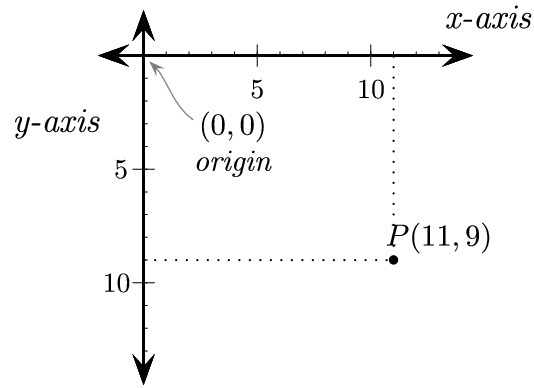
\includegraphics[width=0.55\textwidth]{assets/solution_coordinates/coordinates-system.jpeg}
    \caption{Coordinate System}
    \label{fig:coord}
\end{figure}

\section{Project Structure and PDDL Implementation}

The project is organized into two main directories, \texttt{solution\_coordinates} and \texttt{solution\_adjacency}, each containing the necessary files for implementing and testing the respective approaches. Each directory includes a \texttt{domain.pddl} file, which establishes the model's conditions, including predicates and actions specific to the approach. The \texttt{problem-*.pddl} files define the initial conditions and goal states for each test case, allowing us to evaluate the model under various scenarios.

Additionally, each problem has a corresponding \texttt{problem-*.plan} file, which contains the PDDL plan generated by the planner, and a \texttt{problem-*.txt} file, which logs the planner's output, including computational metrics. To efficiently extract and analyze these metrics, we developed a Python script, \texttt{extract\_metrics.py}, which processes the planner logs to provide insights into the computational performance of each approach.

To facilitate the development and testing of our PDDL files, we set up our project using \textbf{Visual Studio Code} with the PDDL extension. We utilized the \textbf{Delfi planner} to execute and evaluate our PDDL models, allowing us to test various scenarios and configurations efficiently.

In this section, we will only explain the \texttt{domain.pddl} implementation of the \textbf{coordinates} approach. The \textbf{adjacencies} approach is similar, except for the configuration of the grid and the movement actions (which are all unified into one \texttt{move} action). In the next section, \textit{Test Cases and Results}, we will show the multiple problem configurations that we have tested and the results attained with each of them.

\subsection{Requirements}
The only PDDL requirements needed in the domain are:
\begin{enumerate}
    \item \texttt{:strips}, which indicates that the domain adheres to the basic action representation of the STRIPS framework.
    \item \texttt{:negative-preconditions}, which enables the use of the \texttt{not()} operator in the preconditions of actions.
\end{enumerate}
\begin{figure}[ht]
    \centering
    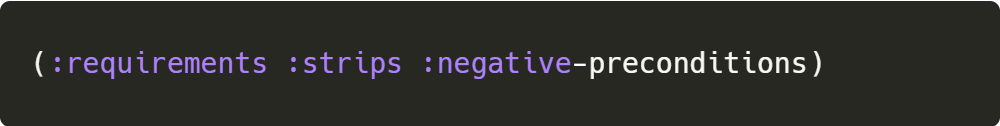
\includegraphics[width=0.55\textwidth]{assets/solution_coordinates/requirements.png}
    \caption{Code: Requirements}
    \label{fig:req}
\end{figure}

\subsection{Predicates}
The predicates are essentially variables that can take either a \textit{true} or \textit{false} value for each collection of \textit{parameters} that they are given. In our domain, the predicates are those discussed in Section~\ref{sec:pred}.
\begin{figure}[ht]
    \centering
    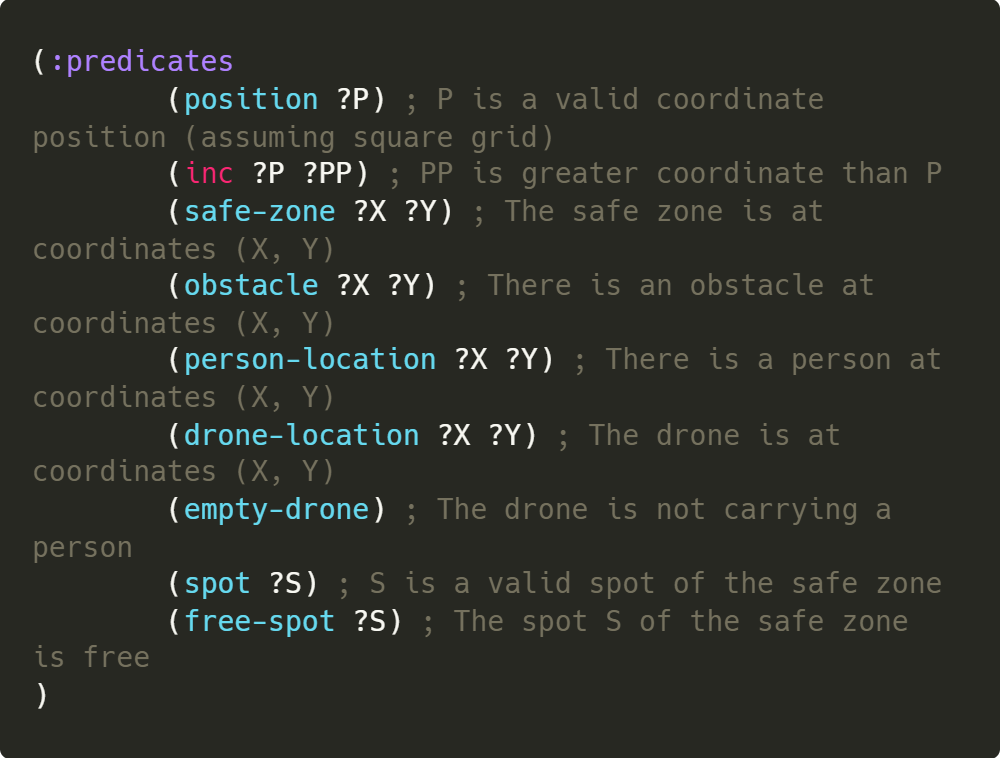
\includegraphics[width=0.55\textwidth]{assets/solution_coordinates/predicates.png}
    \caption{Code: Predicates}
    \label{fig:pred}
\end{figure}

\subsection{Actions}
The actions are the possible steps that can be taken throughout a plan. Each of them recieves a number of \textit{parameters}, which are the objects that intervene in the action. Then, for the action to be allowed to happen, all of its \textit{preconditions} have to be met and, in that case, the \textit{effects} of the action can be applied. In our domain, the actions are those discussed in Section~\ref{sec:act}.
\subsubsection{Movement}
All of the movement actions (\texttt{up}, \texttt{down}, \texttt{right} and \texttt{left}) are very similar, so we will only delve into one of them: the \texttt{up} action, which moves the drone from the current cell of the grid to the one on top.
\begin{itemize}
    \item \underline{Parameters:}
    \begin{itemize}
        \item $X$: Starting X coordinate of the drone.
        \item $Y$: Starting Y coordinate of the drone.
        \item $NY$: New Y coordinate to which the drone is moving.
    \end{itemize}
    \item \underline{Preconditions:}
    \begin{itemize}
        \item \textit{Position(X), Position(Y), Position(NY)}: $X, Y,$ and $NY$ must be valid positions of the grid.
        \item \textit{Inc(NY, Y)}: Since the drone is moving up, NY must be a lower coordinate value than Y.
        \item \textit{Drone-location(X, Y)}: The drone must be at the starting location $(X, Y)$.
        \item \textit{¬Obstacle(X, NY)}: There must \textbf{not} be an obstacle at the new location $(X, NY)$.
    \end{itemize}
    \item \underline{Effects:}
    \begin{itemize}
        \item \textit{Drone-location(X, NY)}: The drone is now at the new location $(X, NY)$.
        \item \textit{¬Drone-location(X, Y)}: The drone is no longer at the starting location $(X, Y)$.
    \end{itemize}
\end{itemize}
\begin{figure}[ht]
    \centering
    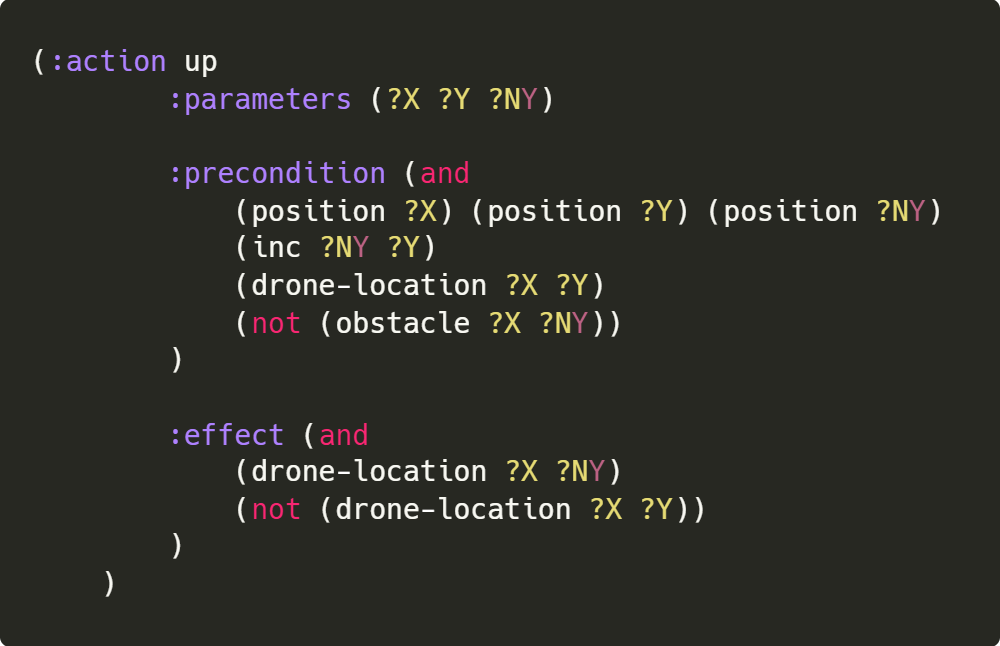
\includegraphics[width=0.55\textwidth]{assets/solution_coordinates/up.png}
    \caption{Code: Up Action}
    \label{fig:act:up}
\end{figure}
The rest of the movement actions (\texttt{down}, \texttt{right} and \texttt{left}) are analog to this one, changing when necessary the order of the increment of coordinates and the new coordinate (from $NY$ to $NX$).

\subsubsection{Pick-up}
The \texttt{pick-up} action places a person from the grid on the drone, for it to carry them to the safe zone.
\begin{itemize}
    \item \underline{Parameters:}
    \begin{itemize}
        \item $X$: Current X coordinate of the drone.
        \item $Y$: Current Y coordinate of the drone.
    \end{itemize}
    \item \underline{Preconditions:}
    \begin{itemize}
        \item \textit{Position(X), Position(Y)}: $X$ and $Y$ must be valid positions of the grid.
        \item \textit{Drone-location(X, Y)}: The drone must be at the location $(X, Y)$.
        \item \textit{Person-location(X, Y)}: A person must be at the location $(X, Y)$.
        \item \textit{Empty-drone()}: The drone must be empty (not carrying anyone).
    \end{itemize}
    \item \underline{Effects:}
    \begin{itemize}
        \item \textit{¬Person-location(X, Y)}: The person is no longer at location $(X, Y)$, they are inside the drone.
        \item \textit{¬Empty-drone()}: The drone is no longer empty.
    \end{itemize}
\end{itemize}
\begin{figure}[ht]
    \centering
    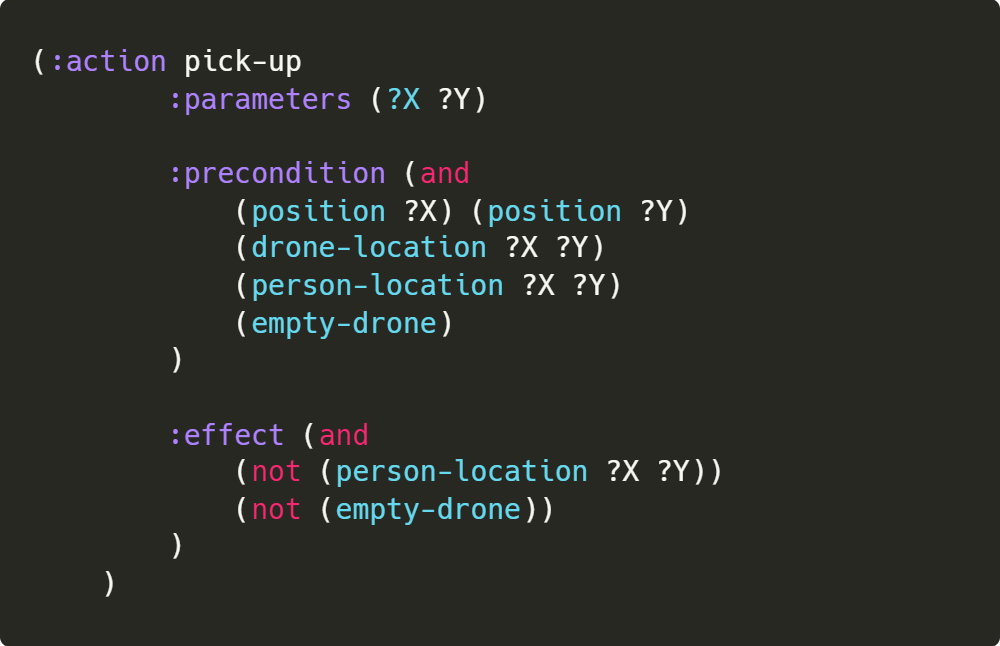
\includegraphics[width=0.55\textwidth]{assets/solution_coordinates/pick-up.png}
    \caption{Code: Pick-Up Action}
    \label{fig:act:pick-up}
\end{figure}

\subsubsection{Drop-off}
The \texttt{drop-off} action leaves a person who is inside the drone at the safe zone.
\begin{itemize}
    \item \underline{Parameters:}
    \begin{itemize}
        \item $X$: Current X coordinate of the drone.
        \item $Y$: Current Y coordinate of the drone.
        \item $S$: One of the spots of the safe zone.
    \end{itemize}
    \item \underline{Preconditions:}
    \begin{itemize}
        \item \textit{Position(X), Position(Y)}: $X$ and $Y$ must be valid positions of the grid.
        \item \textit{Drone-location(X, Y)}: The drone must be at the location $(X, Y)$.
        \item \textit{¬Empty-drone()}: The drone must be carrying a person.
        \item \textit{Safe-Zone(X, Y)}: The safe zone must be at the location $(X, Y)$.
        \item \textit{Spot(S), Free-Spot(S)}: $S$ must be a valid spot of the safe zone, and be free at the moment.
    \end{itemize}
    \item \underline{Effects:}
    \begin{itemize}
        \item \textit{Empty-drone()}: The drone is no longer carrying the person.
        \item \textit{Person-location(X, Y)}: The person is now at location $(X, Y)$, in the safe zone.
        \item \textit{¬Free-Spot(S)}: The spot $S$ of the safe zone is now occupied.
    \end{itemize}
\end{itemize}
\begin{figure}[H]
    \centering
    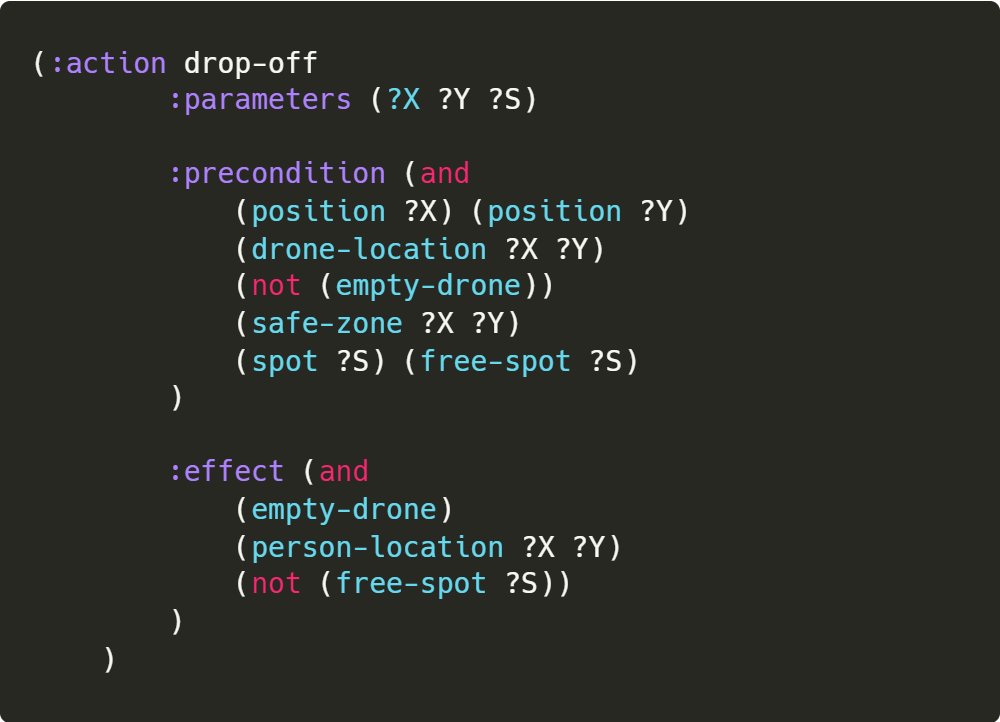
\includegraphics[width=0.55\textwidth]{assets/solution_coordinates/drop-off.png}
    \caption{Code: Drop-Off Action}
    \label{fig:act:drop-off}
\end{figure}

\subsubsection{Evacuate-Safe-Zone}
The \texttt{evacuate-safe-zone} action frees up one of the spots of the safe zone when it is full.
\begin{itemize}
    \item \underline{Parameters:}
    \begin{itemize}
        \item $S$: One of the spots of the safe zone.
    \end{itemize}
    \item \underline{Preconditions:}
    \begin{itemize}
        \item \textit{Spot(S)}: $S$ must be a valid spot of the safe zone.
        \item \textit{¬Free-Spot(S)}: $S$ must be occupied at the moment.
    \end{itemize}
    \item \underline{Effects:}
    \begin{itemize}
        \item \textit{Free-Spot(S)}: The spot $S$ of the safe zone is now free.
    \end{itemize}
\end{itemize}
\begin{figure}[ht]
    \centering
    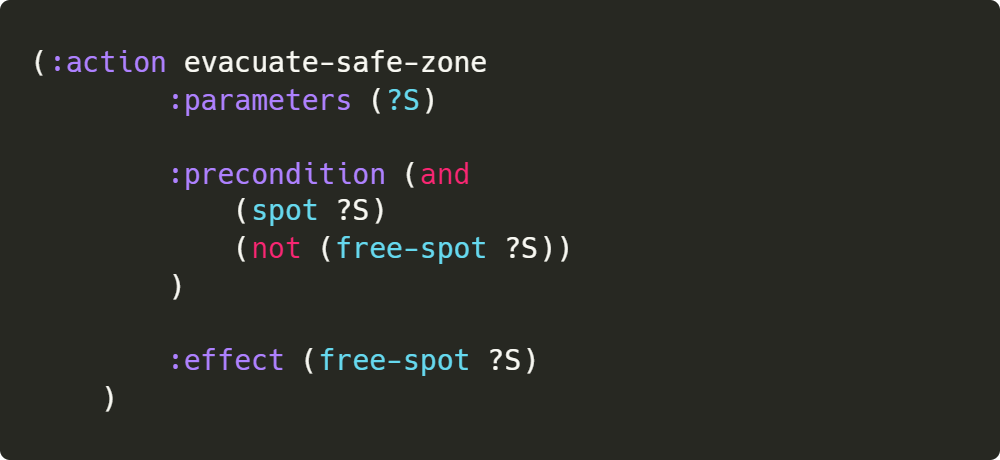
\includegraphics[width=0.55\textwidth]{assets/solution_coordinates/evacuate-safe-zone.png}
    \caption{Code: Evacuate-Safe-Zone Action}
    \label{fig:act:evacuate}
\end{figure}

\section{Test Cases and Results}

We conducted tests on a total of seven cases, each with increasing complexity. We began with a very basic scenario to verify the core functionality of the model and concluded with an unsolvable case that highlights the limitations of the established rules.

For each of the seven cases, we briefly explain the objective of that test case, display a diagram of the initial and goal states.

% For each of the 7 cases, we briefly explain the objective of that test case, display a diagram of the initial and goal states, and then show the \textit{PDDL} implementation of the problem.

\subsection{Case 1: Basic}

To begin, we tested the fundamental functionalities of the model, focusing on the drone's basic movement and carrying actions. This initial test case features a small \(3 \times 3\) grid with no obstacles and a number of people that can comfortably fit into the safe zone.

\begin{figure}[ht]
    \centering
    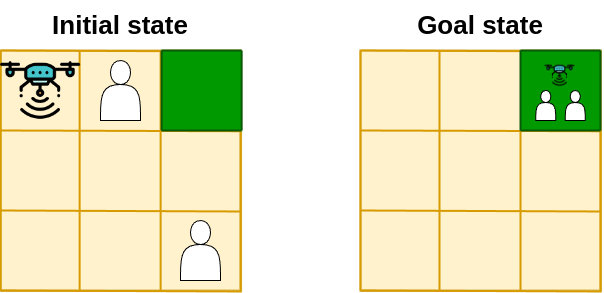
\includegraphics[width=0.55\textwidth]{assets/problem-1-basic.drawio.png}
    \caption{Case 1: Basic}
    \label{fig:initial-state}
\end{figure}

\subsubsection{Solution}
We can see that the movement actions function correctly with the coordinate system we have built for the model, as well as the pick-up and drop-off actions.

\subsection{Case 2: Basic with Obstacles}

Subsequently, we incorporate an additional complexity into the model: the presence of obstacles. This scenario replicates the conditions of Case 1, utilizing a small grid and a number of individuals that can be accommodated within the safe zone. However, an obstacle is strategically positioned in the direct path between one of the individuals and the safe zone. This setup is designed to rigorously assess the drone's navigational algorithms and its ability to effectively circumvent obstacles.

\begin{figure}[H]
    \centering
    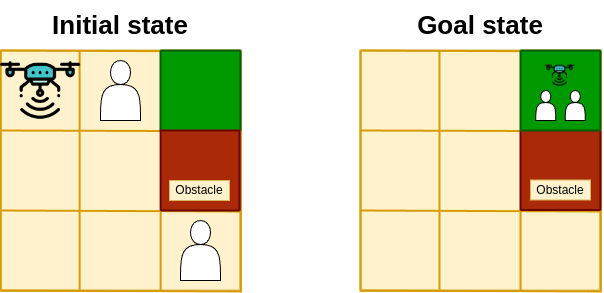
\includegraphics[width=0.55\textwidth]{assets/problem-2-basic-obstacle.drawio.png}
    \caption{Case 2: Basic with Obstacles}
    \label{fig:initial-state-obstacles}
\end{figure}

\subsubsection{Solution}
We now see that the obstacles also act as expected, impeding the movement actions through the cells they occupy. This makes the drone avoid the obstacle by moving around it.

\subsection{Case 3: Overcrowded}

For the next case, we examine another of the features of the model: the capacity of the safe zone. In order to do this, we again utilize a simple layout with a small grid and no obstacles, but in this case, we introduce one more person to rescue, which makes the total number of people bigger than the safe zone capacity. The goal of this test case is to study whether the “spots” feature of the safe zone works as expected.

\begin{figure}[H]
    \centering
    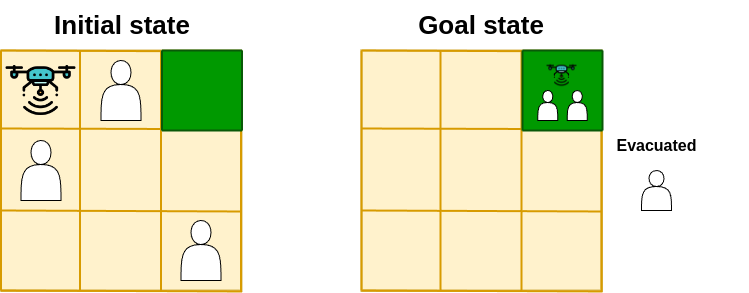
\includegraphics[width=0.55\textwidth]{assets/problem-3-overcrowded.drawio.png}
    \caption{Case 3: Overcrowded}
    \label{fig:initial-state-overcrowded}
\end{figure}

\subsubsection{Solution}
In this case, we prove that the safe zone capacity is being taken into account as it should, having to evacuate one of the spots before dropping off the last person at the safe zone.

\textbf{Note}: On earlier iterations of the model, we tried to implement the safe zone capacity with numeric functions (\texttt{:fluents} requirement of PDDL), but the available free online planners have trouble supporting them. Therefore, the concept of the spots of the free zone was implemented as a clean way to keep a count of the amount of people in the safe zone by only using predicates and actions (no functions)

\subsection{Case 4: Default (PDF example)}

For case 4, we evaluate the default scenario provided as an example in the assignment. This configuration involves rescuing three individuals and navigating around three obstacles within a \(4 \times 4\) grid. This test case is designed to assess nearly all aspects of the model's functionality within a slightly larger grid than previous scenarios.

\begin{figure}[ht]
    \centering
    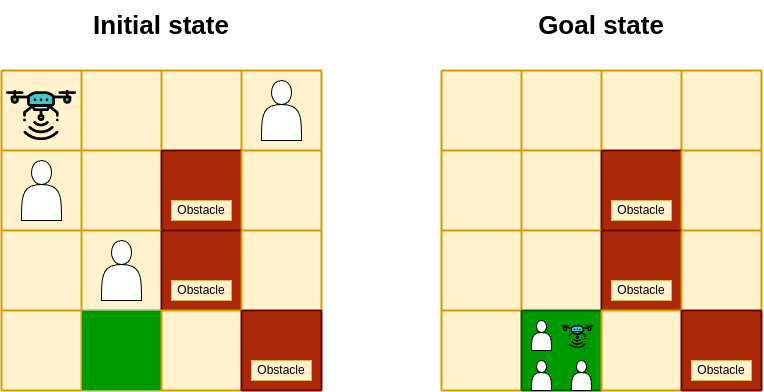
\includegraphics[width=0.55\textwidth]{assets/problem-4-pdf-example.drawio.png}
    \caption{Case 4: Default (PDF example)}
    \label{fig:initial-state-default}
\end{figure}

\subsubsection{Solution}
It is now shown that we can easily enlarge the problem from a 3x3 to a 4x4 grid and the model still functions as expected.

\subsection{Case 5: Bigger Grid}

We proceed to conduct a test on a larger grid, specifically a \(5 \times 5\) configuration. This scenario includes five obstacles and six individuals requiring rescue, resulting in a situation where the number of people exceeds the available spots in the safe zone. This comprehensive test case is designed to evaluate all functionalities of the model within a single scenario.

\begin{figure}[ht]
    \centering
    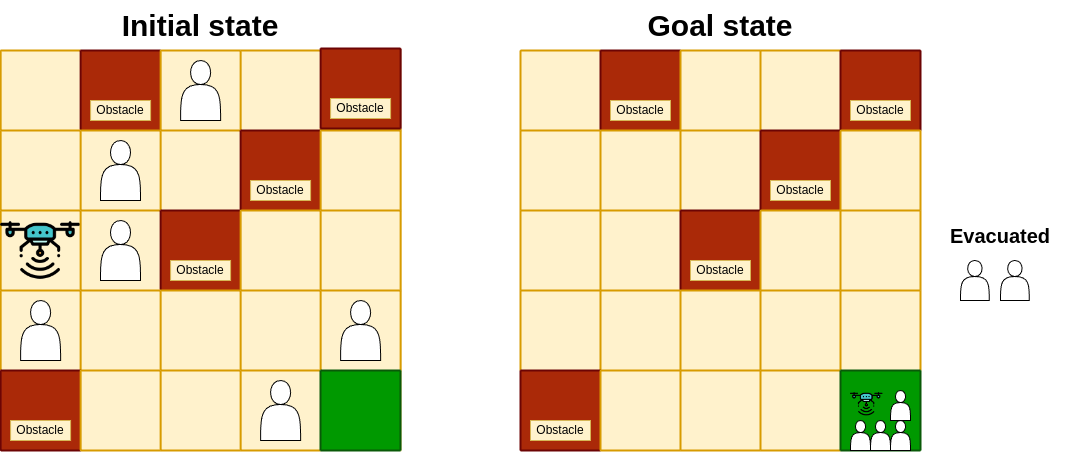
\includegraphics[width=0.55\textwidth]{assets/problem-5-big.drawio.png}
    \caption{Case 5: Bigger Grid}
    \label{fig:initial-state-bigger-grid}
\end{figure}

\subsubsection{Solution}
Here we can appreciate how the most comprehensive test case (which includes all of the functionalities of the model) is solved correctly.

\subsection{Case 6: Maze}

With this test case, we aim to again display all of the functionalities of the model, but this time in a neat and visual scenario that simulates a maze.

\begin{figure}[ht]
    \centering
    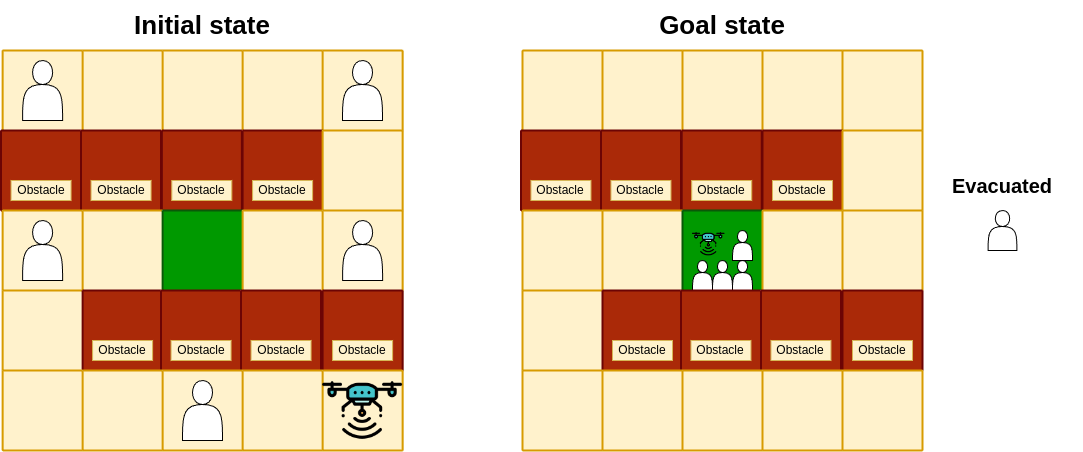
\includegraphics[width=0.55\textwidth]{assets/problem-6-maze.drawio.png} % Increased width
    \caption{Case 6: Maze}
    \label{fig:initial-state-maze}
\end{figure}

\subsubsection{Solution}
We check again with a different test case that all of the functionalities behave as they should.

\subsection{Case 7: Impossible}

Finally, as a way to showcase the limits and restrictions of the model, we introduce a test case which is unsolvable. In this layout, the safe zone is fully surrounded by obstacles, and the only possible way to access it might be by moving diagonally, which is currently not an allowed type of movement.

\begin{figure}[H]
    \centering
    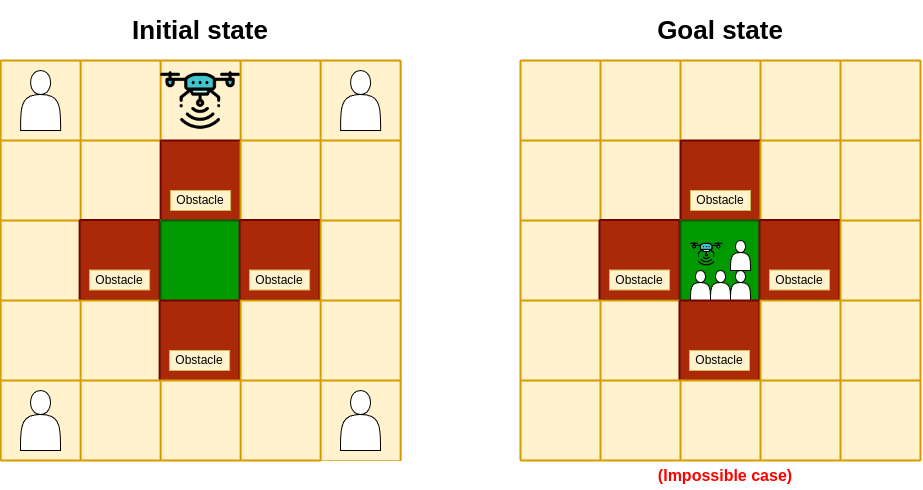
\includegraphics[width=0.55\textwidth]{assets/problem-7-impossible.drawio.png} % Increased width
    \caption{Case 7: Impossible}
    \label{fig:initial-state-impossible}
\end{figure}

\subsubsection{Solution}
Finally, we see how the planner indeed cannot find a solution to the proposed problem, which was the expected outcome, given that it should be impossible to solve with the given set of rules of the model

\section{Performance Analysis}

The following table summarizes the results of the test cases, comparing the performance metrics for the "Adjacency" and "Coordinates" approaches across different problems.

\begin{table}[ht]
    \centering
    \small
    \begin{tabular}{|c|l|c|c|c|c|}
        \hline
        \textbf{Problem} & \textbf{Method} & \textbf{Plan Cost} & \textbf{Nodes Generated} & \textbf{Nodes Expanded} & \textbf{Total Time} \\
        \hline
        \multirow{2}{*}{Problem-1} & Adjacency & 10 & 0 & 0 & 0.28 \\
                                   & Coordinates & 10 & 0 & 0 & 0.38 \\
        \hline
        \multirow{2}{*}{Problem-2} & Adjacency & 14 & 0 & 0 & 0.10 \\
                                   & Coordinates & 14 & 0 & 0 & 0.14 \\
        \hline
        \multirow{2}{*}{Problem-3} & Adjacency & 17 & 72 & 24 & 0.0308 \\
                                   & Coordinates & 17 & 57 & 18 & 0.1754 \\
        \hline
        \multirow{2}{*}{Problem-4} & Adjacency & 22 & 77 & 23 & 0.0320 \\
                                   & Coordinates & 22 & 725 & 248 & 1.6226 \\
        \hline
        \multirow{2}{*}{Problem-5} & Adjacency & 62 & 233 & 63 & 0.0172 \\
                                   & Coordinates & 62 & 46715 & 16940 & 1.8306 \\
        \hline
        \multirow{2}{*}{Problem-6} & Adjacency & 51 & 138 & 52 & 0.0149 \\
                                   & Coordinates & 51 & 10631 & 4749 & 3.9974 \\
        \hline
        \multirow{2}{*}{Problem-7} & Adjacency & - & 0 & 0 & 0.0007 \\
                                   & Coordinates & - & 0 & 0 & 0.0009 \\
        \hline
    \end{tabular}
    \caption{Comparison of performance metrics for different solutions and problems.}
    \label{tab:results}
\end{table}

The table evaluates the following several key performance metrics for each approach:

\begin{itemize}
    \item \textbf{Plan Cost:} Represents the cumulative cost of executing all actions in a plan. Lower costs indicate more efficient solutions.
    
    \item \textbf{Nodes Generated:} Provides insight into the computational effort of the search algorithm by indicating the total number of states considered.
    
    \item \textbf{Nodes Expanded:} Shows how many of the generated states were fully explored, offering a measure of the search's thoroughness.
    
    \item \textbf{Total Time:} Reflects the duration taken by the algorithm to find a solution. Faster times are advantageous, especially in time-sensitive scenarios.
\end{itemize}

Our results provide a comparative analysis of the "Adjacency" and "Coordinates" approaches across several problems. The Plan Cost remains consistent across both approaches for each problem, indicating that both methods are equally effective in terms of the cost of executing actions. Notably, in Problems 1 and 2, the metrics for Nodes Generated and Nodes Expanded are both zero. This suggests that these problems are straightforward enough that the initial state is already close to the goal state, requiring minimal exploration of the search space. Consequently, the search algorithms can directly reach the solution without generating or expanding additional nodes. However, as the complexity of the problems increases, the "Coordinates" approach generally generates and expands more nodes than the "Adjacency" approach, particularly noticeable in Problems 4 and 5. This indicates that the "Coordinates" method explores a larger search space, which could imply a more thorough search and therefore more computational effort. Interestingly, in Problem 3, the "Coordinates" solution generated and expanded fewer nodes than the "Adjacency" approach, yet it was still significantly slower. This highlights a potential inefficiency in the "Coordinates" method, where even with fewer nodes, the time taken is longer. The Total Time metric consistently shows that the "Coordinates" approach often takes longer to find a solution compared to the "Adjacency" approach. This is especially evident as the complexity of the problems increases, where the time difference becomes more pronounced. Overall, the "Adjacency" approach appears to be more efficient in terms of computational resources and time, particularly as the complexity of the problem evolves.

\section{Conclusion}

In this report, we explored two distinct approaches for modeling a rescue drone tasked with saving individuals in an emergency grid environment: the "Adjacency List" and the "Coordinate System" methods. Through a series of test cases, we evaluated the performance of each approach in terms of Plan Cost, Nodes Generated, Nodes Expanded, and Total Time.

\vspace{1em}

Our analysis revealed that while both approaches achieve optimal Plan Costs, the "Adjacency List" method consistently outperforms the "Coordinate System" in terms of computational efficiency, particularly as the complexity of the problems increases. This is evidenced by the lower number of nodes generated and expanded, as well as the reduced total time required to find solutions. The "Coordinate System" approach, although more concise in its problem definition, tends to explore a larger search space, leading to increased computational effort and time.

\vspace{1em}

Interestingly, in simpler scenarios such as Problems 1 and 2, both methods required minimal exploration, resulting in zero nodes generated and expanded. However, as the complexity increased, the "Adjacency List" approach demonstrated superior efficiency, making it a more suitable choice for complex problem-solving scenarios.

\vspace{1em}

This study emphasizes the importance of selecting the right modeling approach based on the specific needs and constraints of the problem to achieve the best results effectively and efficiently. Additionally, exploring the use of fluents or comparing our methods with other planners could provide further insights and improvements.

\end{document}